%===================================== CHAP 4 =================================

\chapter{Requirements engineering}

The requirements engineering process was a continuous negotiation between the customer and the development team. Although the customer had a solid understanding of what they wanted, this process went on throughout the duration of the project.

Furthermore, requirements are separated into two categories. A functional requirement describes a function of the system or one of it's components. On the other hand, a non-functional requirement can be viewed with regards to the operation of the system. Rather than listing specific functions of the system, it describes the performance or operation of the system as a whole.

\section{Requirements elicitation}

The functional requirements were elicited as a result of discussion both within the group and with the customer. Use cases and stories were used as help to define the exact requirements and formulations of them. The use cases describe the steps that needed to be performed in order to accomplish a certain task. The result of the process was a list, describing the requirements and the prioritization of them.

The non-functional requirements were purely a result of discussion with the customer. After identifying the properties of the system, they were classified and rated in order of importance.

Two issues arose when requirements for the different protocols were to be defined. First of all, the customer wanted as many protocols to be implemented as possible. After considering the time available, the three most important protocols were listed as requirements. The decision was subject to change however, depending on how much time it would take to implement each protocol.

The other issue was defining the protocols as requirements. On the one hand, they could be seen as functional requirements. As a user, one must be able to send a message using protocol "A". This would be regarded as a functional requirement. On the other hand, a protocol could be viewed as a property of the system. The protocol would then be considered a set of standards the system has to support, and fall under the compatibility category of non-functional requirements. The functional requirements would then only be described as a user being able to send a message, regardless of protocol. The decision wouldn't make a difference to the product, so extensive  research into this definition was discarded.

\section{Functional requirements}

After a brief evaluation, the different protocols were defined as functional requirements. Mainly due to a consideration of how they would be tested. It seemed more reasonable to include them as functional requirements when considering the integration testing of components, as well as acceptance testing. The other functional requirements were concerned with what a user was supposed to do with the user interface. The general goal of the interface was to expose configuration of mappings between supported protocols, publisher and subscriber database listings, as well as topics and content filters. The functional requirements are described in table \ref{func-requirements}, and was a result of the requirements elicitation process.

The protocols were viewed as the most important requirements, as they were the core function of the system. The log in function was not as important. One does not strictly need a log in function in such a system, due to the fact that you only get access to the local instance and database. The function serves as a security measure, in case one accidentally leaves the computer unlocked, or some similar case occurs.

\begin{table}[ht!]
\centering
\resizebox{9cm}{!}{
\begin{tabular}{|l|l|p{5cm}|l|}
\hline
\multicolumn{4}{|c|}{\textbf{Functional requirements}}  \\ \hline
\multicolumn{1}{|c|}{\textbf{$\#$}} & \textbf{Use Case} & \textbf{Description}    & \textbf{Priority} \\ \hline
\multicolumn{1}{|c|}{FR1.1} & \multicolumn{1}{c|}{U5, U6} & A user must be able to send and receive messages over the WSN protocol. & 
\multicolumn{1}{c|}{1} \\ \hline
\multicolumn{1}{|c|}{FR1.2} & \multicolumn{1}{c|}{??} & A user must be able to subscribe to a topic using the WSN protocol &
\multicolumn{1}{c|}{1} \\ \hline
\multicolumn{1}{|c|}{FR1.3} & \multicolumn{1}{c|}{??} & A user must be able to register as a publisher on a topic using the WSN protocol &
\multicolumn{1}{c|}{1} \\ \hline
\multicolumn{1}{|c|}{FR1.4} & \multicolumn{1}{c|}{??} & A user must be able to unsubscribe from a topic using the WSN protocol &
\multicolumn{1}{c|}{1} \\ \hline
\multicolumn{1}{|c|}{FR1.5} & \multicolumn{1}{c|}{??} & A user must be able to unregister as a publisher on a topic using the WSN protocol &
\multicolumn{1}{c|}{1} \\ \hline
\multicolumn{1}{|c|}{FR1.6} & \multicolumn{1}{c|}{??} & A must be able to retrieve the latest message on a topic using the GetCurrentMessage function using the WSN protocol &
\multicolumn{1}{c|}{1} \\ \hline
\multicolumn{1}{|c|}{FR1.7} & \multicolumn{1}{c|}{??} & A user must be able to renew his/her subscription using the WSN protocol &
\multicolumn{1}{c|}{1} \\ \hline
\multicolumn{1}{|c|}{FR1.8} & \multicolumn{1}{c|}{??} & A user must be able to pause his/her subscription using the WSN protocol &
\multicolumn{1}{c|}{1} \\ \hline
\multicolumn{1}{|c|}{FR1.9} & \multicolumn{1}{c|}{??} & A user must be able to resume his/her subscription using the WSN protocol &
\multicolumn{1}{c|}{1} \\ \hline
\multicolumn{1}{|c|}{FR1.10} & \multicolumn{1}{c|}{??} & A user must be able to send multiple notification messages in a single Notify using the WSN protocol &
\multicolumn{1}{c|}{1} \\ \hline
\multicolumn{1}{|c|}{FR2} & \multicolumn{1}{c|}{U5 \& U6} & A user must be able to send and recieve messages using the AMQP protocol &
\multicolumn{1}{c|}{1} \\ \hline
\multicolumn{1}{|c|}{FR3} & \multicolumn{1}{c|}{U1} & The admin must be able to map topics/dialects with other topics. &
\multicolumn{1}{c|}{2} \\ \hline
\multicolumn{1}{|c|}{FR4} & \multicolumn{1}{c|}{U2} & The admin must be able to edit the different subscriptions. That means delete one or all subscriptions on a given topic. This also includes deleting all topics. & \multicolumn{1}{c|}{3} \\ \hline
\multicolumn{1}{|c|}{FR5} & \multicolumn{1}{c|}{U3} & The admin should be able to get information in the administrator interface about the server. &  \multicolumn{1}{c|}{4} \\ \hline
\multicolumn{1}{|c|}{FR6} & \multicolumn{1}{c|}{U4} & The admin must be able to log in with a user name and password to get access to core functions. & \multicolumn{1}{c|}{5} \\ \hline
\end{tabular}
}
\caption{Functional requirements}
\label{func-requirements}
\end{table}

\clearpage

\section{Non-functional requirements}

Following is a list of the non-functional requirements created. The requirements are listed in descending order of importance. 

\subsection{NFR1 - Extendability}

\subsubsection{NFR1.1 - Modularization}

The different components of the system should be decomposed in such away that the respective components are loosely coupled, to allow easier addition of more protocols at a later point in time. It also allows upgrading and further developing of different parts of the system individually.

\subsubsection{NFR1.2 - Protocol independency}

The system must be able to translate between protocols independent of their type, more precisely it must not only support to/from WSN, but also between protocols like AMQP and MQTT, without having to go through WSN.

\subsection{NFR2 - Documentation}

All parts of the application must be documented according to the language specific standards, preferably in English.

\subsection{NFR3 - Open Source}

The software shall be open source. The software shall be available for use, change and distribution by anyone. It will be licenced under the MiT licence.

\section{User stories}

The following table describes the user stories defined. The stories were used as a tool to create use cases. The stories were defined based on conversations with the customer, and answers to what the customer wanted to do with the system. The different aspects were then structured in the following table.

\clearpage

\begin{table}[ht!]
\centering
\begin{tabular}{|l|p{5cm}|p{3cm}|}
\hline
\multicolumn{3}{|c|}{\textbf{User stories}} \\ \hline
\textbf{As a(n)} & \textbf{I want to} & \textbf{So that (I can)}  \\ \hline
Admin & Log in with username and password. & Gain access to the system. \\ \hline
Admin & Get information about server. & See number of subscribers and system status.  \\ \hline
Admin & Get information about subscribers. & See number of connections to the broker.  \\ \hline
Admin & Get server information. & See which IP the broker is running on. \\ \hline
Admin & Get IP and topics information. & See information about subscribers and topics. \\ \hline
Admin & Get resource overview. & See load and balance of the server. \\ \hline
Admin & Edit topics/dialects. & Map topics/dialects. \\ \hline
Admin & Edit subscriptions. & Unsubscribe users on topics. \\ \hline
Admin & Edit topics. & Delete a topic. \\ \hline
User & Send a message over WSN. & Publish information. \\ \hline
User & Send a message over AMQP. & Publish information. \\ \hline
User & Receive a message over WSN. & Receive information from other units. \\ \hline
User & Receive a message over AMQP. & Receive information from other units. \\ \hline
\end{tabular}
\caption{User stories}
\label{user-stories}
\end{table}

\clearpage

\section{Use cases}

The use cases constructed for this project were used as a tool to create the requirements. They were also used for internal communication within the group, as a simple way to share information about the user interface. The use cases regarding the protocols were combined into one, as they are the same for all of them.

\subsection{Use case 1 - Topic mapping}

Below is the use case for the topic mapping part of the interface. The main goal is to administer the topics. After (and/or before) a publisher has added a topic, it must be able to map this topic to another topic. It should also be possible to create links and set flags on topics (dialect for WSN).

\begin{table}[ht!]
\begin{minipage}{.6\textwidth}
\centering
\resizebox{\textwidth}{!}{
\begin{tabular}{|l|p{5cm}|}
\hline
\textbf{Use case ID} & U1 \\ \hline
\textbf{Use case Name} & Topic mapping \\ \hline
\textbf{Description} & Admin should be able to map between topics.  \\ \hline
\textbf{Pre conditions} & The admin is logged in.\\ \hline
\textbf{Standard flow} & \begin{enumerate}
\item Click the config pane.
\item Click on the topic to be mapped.
\item Enter the topic to map against.
\item Click the "Add"-button.
\end{enumerate} \\ \hline
\textbf{Alternative flow} & \begin{description}
\item[2A:] Server won't answer request  \begin{enumerate}
\item Display error message.
\item Open config file for topic mapping.
\item Edit file with the mapping.
\item Save config file.
\item Restart/reload server.
\end{enumerate}
\end{description} \\ \hline
\textbf{Post conditions} & Subscribers of different topics now receives a notify when a publisher publishes on one of the topics.  \\ \hline
\end{tabular}
}
\caption{Use case 1 - Topic mapping}
\label{uc1}
\end{minipage}
\hfill
\begin{minipage}{.4\textwidth}
\centering
\begin{center}
    \makebox[\textwidth]{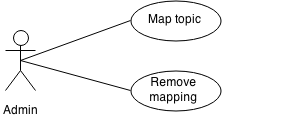
\includegraphics[width=\textwidth]{fig/usecase/usecase_v3_map.png}}
    \caption{U1 - Topic mapping}
    \label{fig:u1}
\end{center}
\end{minipage}
\end{table}

\clearpage

\subsection{Use case 2 - Topic handling}

This use case describes how an administrator can edit topics. The administrator must be able to delete one or all subscriptions on a topic. Deletion of topics is also included in the use case.

\begin{table}[ht!]
\centering
\begin{tabular}{|l|p{5cm}|}
\hline
\textbf{Use case ID} & U2 \\ \hline
\textbf{Use case Name} & Topic handling \\ \hline
\textbf{Description} & Admin should be able to delete topics.  \\ \hline
\textbf{Pre conditions} & The admin is logged in and there exists one or more topics. \\ \hline
\textbf{Standard flow} & \begin{enumerate}
\item Click the topics pane.
\item Click the topic to edit.
\item Alternatives: \begin{enumerate}
    \item Delete one topic.
    \item Delete one subscriber.
    \item Delete all topics.
\end{enumerate}
\end{enumerate} \\ \hline
\textbf{Alternative flow} &  \\ \hline
\textbf{Post conditions} & Subscribers or topics are deleted from the broker.  \\ \hline
\end{tabular}
\caption{Use case 2 - Topic handling}
\label{uc2}
\end{table}

\begin{center}
  \begin{figure}[ht!]
    \makebox[\textwidth]{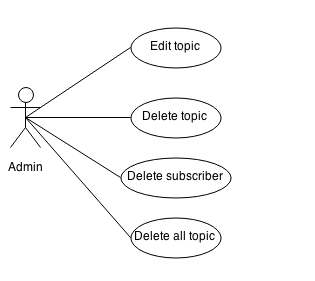
\includegraphics[width=5.5cm]{fig/usecase/usecase_v3_topic.png}}
    \caption{U2 - Topic handling}
    \label{fig:u2}
  \end{figure}
\end{center}

\clearpage

\subsection{Use case 3 - Server information}

This use case describes how an administrator can view information about the server. This includes server statistics and message brokering statistics. 

\begin{table}[ht!]
\centering
\begin{tabular}{|l|p{5cm}|}
\hline
\textbf{Use case ID} & U3 \\ \hline
\textbf{Use case Name} & Server information. \\ \hline
\textbf{Description} & As an admin I would like to see information and status about the server.  \\ \hline
\textbf{Pre conditions} & The admin is logged in.\\ \hline
\textbf{Standard flow} & \begin{enumerate}
\item Click the pane of interest.
\item Read information on the pane of interest.  
\end{enumerate} \\ \hline
\textbf{Alternative flow} & \\ \hline
\textbf{Post conditions} & The admin has seen the information. \\ \hline
\end{tabular}
\caption{Use case 3 - Server information}
\label{uc3}
\end{table}

\begin{center}
  \begin{figure}[ht!]
    \makebox[\textwidth]{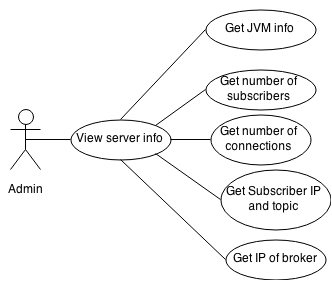
\includegraphics[width=6cm]{fig/usecase/usecase_v3_serverinfo.png}}
    \caption{U3 - Server information}
    \label{fig:u3}
  \end{figure}
\end{center}

\clearpage

\subsection{Use case 4 - Log in}

The following describes the log in procedure. The group concluded that no other functions were needed than a simple username and password log in function. Recover password were not included due to there being little to no persistent data in the database. Thus, a new instance could be initiated instead.

\begin{table}[ht!]
\centering
\begin{tabular}{|l|p{5cm}|}
\hline
\textbf{Use case ID} & U2 \\ \hline
\textbf{Use case Name} & Log in \\ \hline
\textbf{Description} & As an Admin I would like to log in to the admin console. \\ \hline
\textbf{Pre conditions} & The admin is not logged in. \\ \hline
\textbf{Standard flow} & \begin{enumerate}
\item Inserts username and password.
\item Clicks "Log in".
\item Enter the admin console. 
\end{enumerate} \\ \hline
\textbf{Alternative flow} & \begin{description}
\item[2A:] The username or password is wrong. \begin{enumerate}
\item Redirect user to front page.
\item Display error message.
\end{enumerate}
\end{description} \\ \hline
\textbf{Post conditions} & Admin logged in. \\ \hline
\end{tabular}
\caption{Use case 4 - Log in}
\label{uc4}
\end{table}

\begin{center}
  \begin{figure}[ht!]
    \makebox[\textwidth]{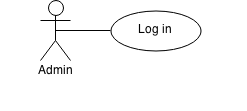
\includegraphics[width=6cm]{fig/usecase/usecase1.png}}
    \caption{U4 - Log in}
    \label{fig:u4}
  \end{figure}
\end{center}

\subsection{Use case 5 - Message sending}

This use case attempts to capture the process of sending messages over the system. This only captures a simplified version of the message sending. Some variations occur from protocol to protocol.

\begin{table}[ht!]
\centering
\begin{tabular}{|l|p{5cm}|}
\hline
\textbf{Use case ID} & U5 \\ \hline
\textbf{Use case Name} & Message sending \\ \hline
\textbf{Description} & User should be able to send a message over a protocol.  \\ \hline
\textbf{Pre conditions} &  \\ \hline
\textbf{Standard flow} & \begin{enumerate}
\item Register as a publisher on a topic.
\item Send the message.
\end{enumerate} \\ \hline
\textbf{Alternative flow} & \begin{enumerate}
\item [1A:] Topic is protected.
\item User registers as publisher with username and password.
\end{enumerate} \\ \hline
\textbf{Post conditions} & Message is sent.  \\ \hline
\end{tabular}
\caption{Use case 5 - Message sending}
\label{uc5}
\end{table}

\begin{center}
  \begin{figure}[ht!]
    \makebox[\textwidth]{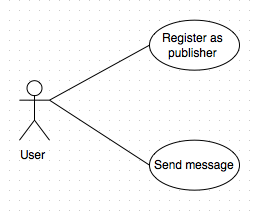
\includegraphics[width=6cm]{fig/usecase/usecase5.png}}
    \caption{U5 - Message sending}
    \label{fig:u5}
  \end{figure}
\end{center}

\subsection{Use case 6 - Message Receiving}

This use case attempts to capture the process of receiving messages over the system. This only captures a simplified version of the message retrieval. Some variations occur from protocol to protocol.

\begin{table}[ht!]
\centering
\begin{tabular}{|l|p{5cm}|}
\hline
\textbf{Use case ID} & U6 \\ \hline
\textbf{Use case Name} & Receiving messages. \\ \hline
\textbf{Description} & User should be able to receive a message over a protocol.  \\ \hline
\textbf{Pre conditions} & The message is sent. \\ \hline
\textbf{Standard flow} & \begin{enumerate}
\item Register as a subscriber on a topic.
\item Receive the message.
\end{enumerate} \\ \hline
\textbf{Alternative flow} & \\ \hline
\textbf{Post conditions} & Message has been received.  \\ \hline
\end{tabular}
\caption{Use case 6 - Message retrieval}
\label{uc6}
\end{table}

\begin{center}
  \begin{figure}[ht!]
    \makebox[\textwidth]{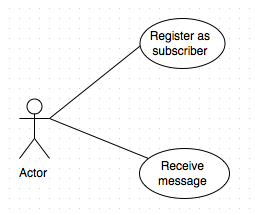
\includegraphics[width=6cm]{fig/usecase/usecase6.png}}
    \caption{U6 - Message retrieval}
    \label{fig:u6}
  \end{figure}
\end{center}

\clearpage